\begin{figure}
    \centering
    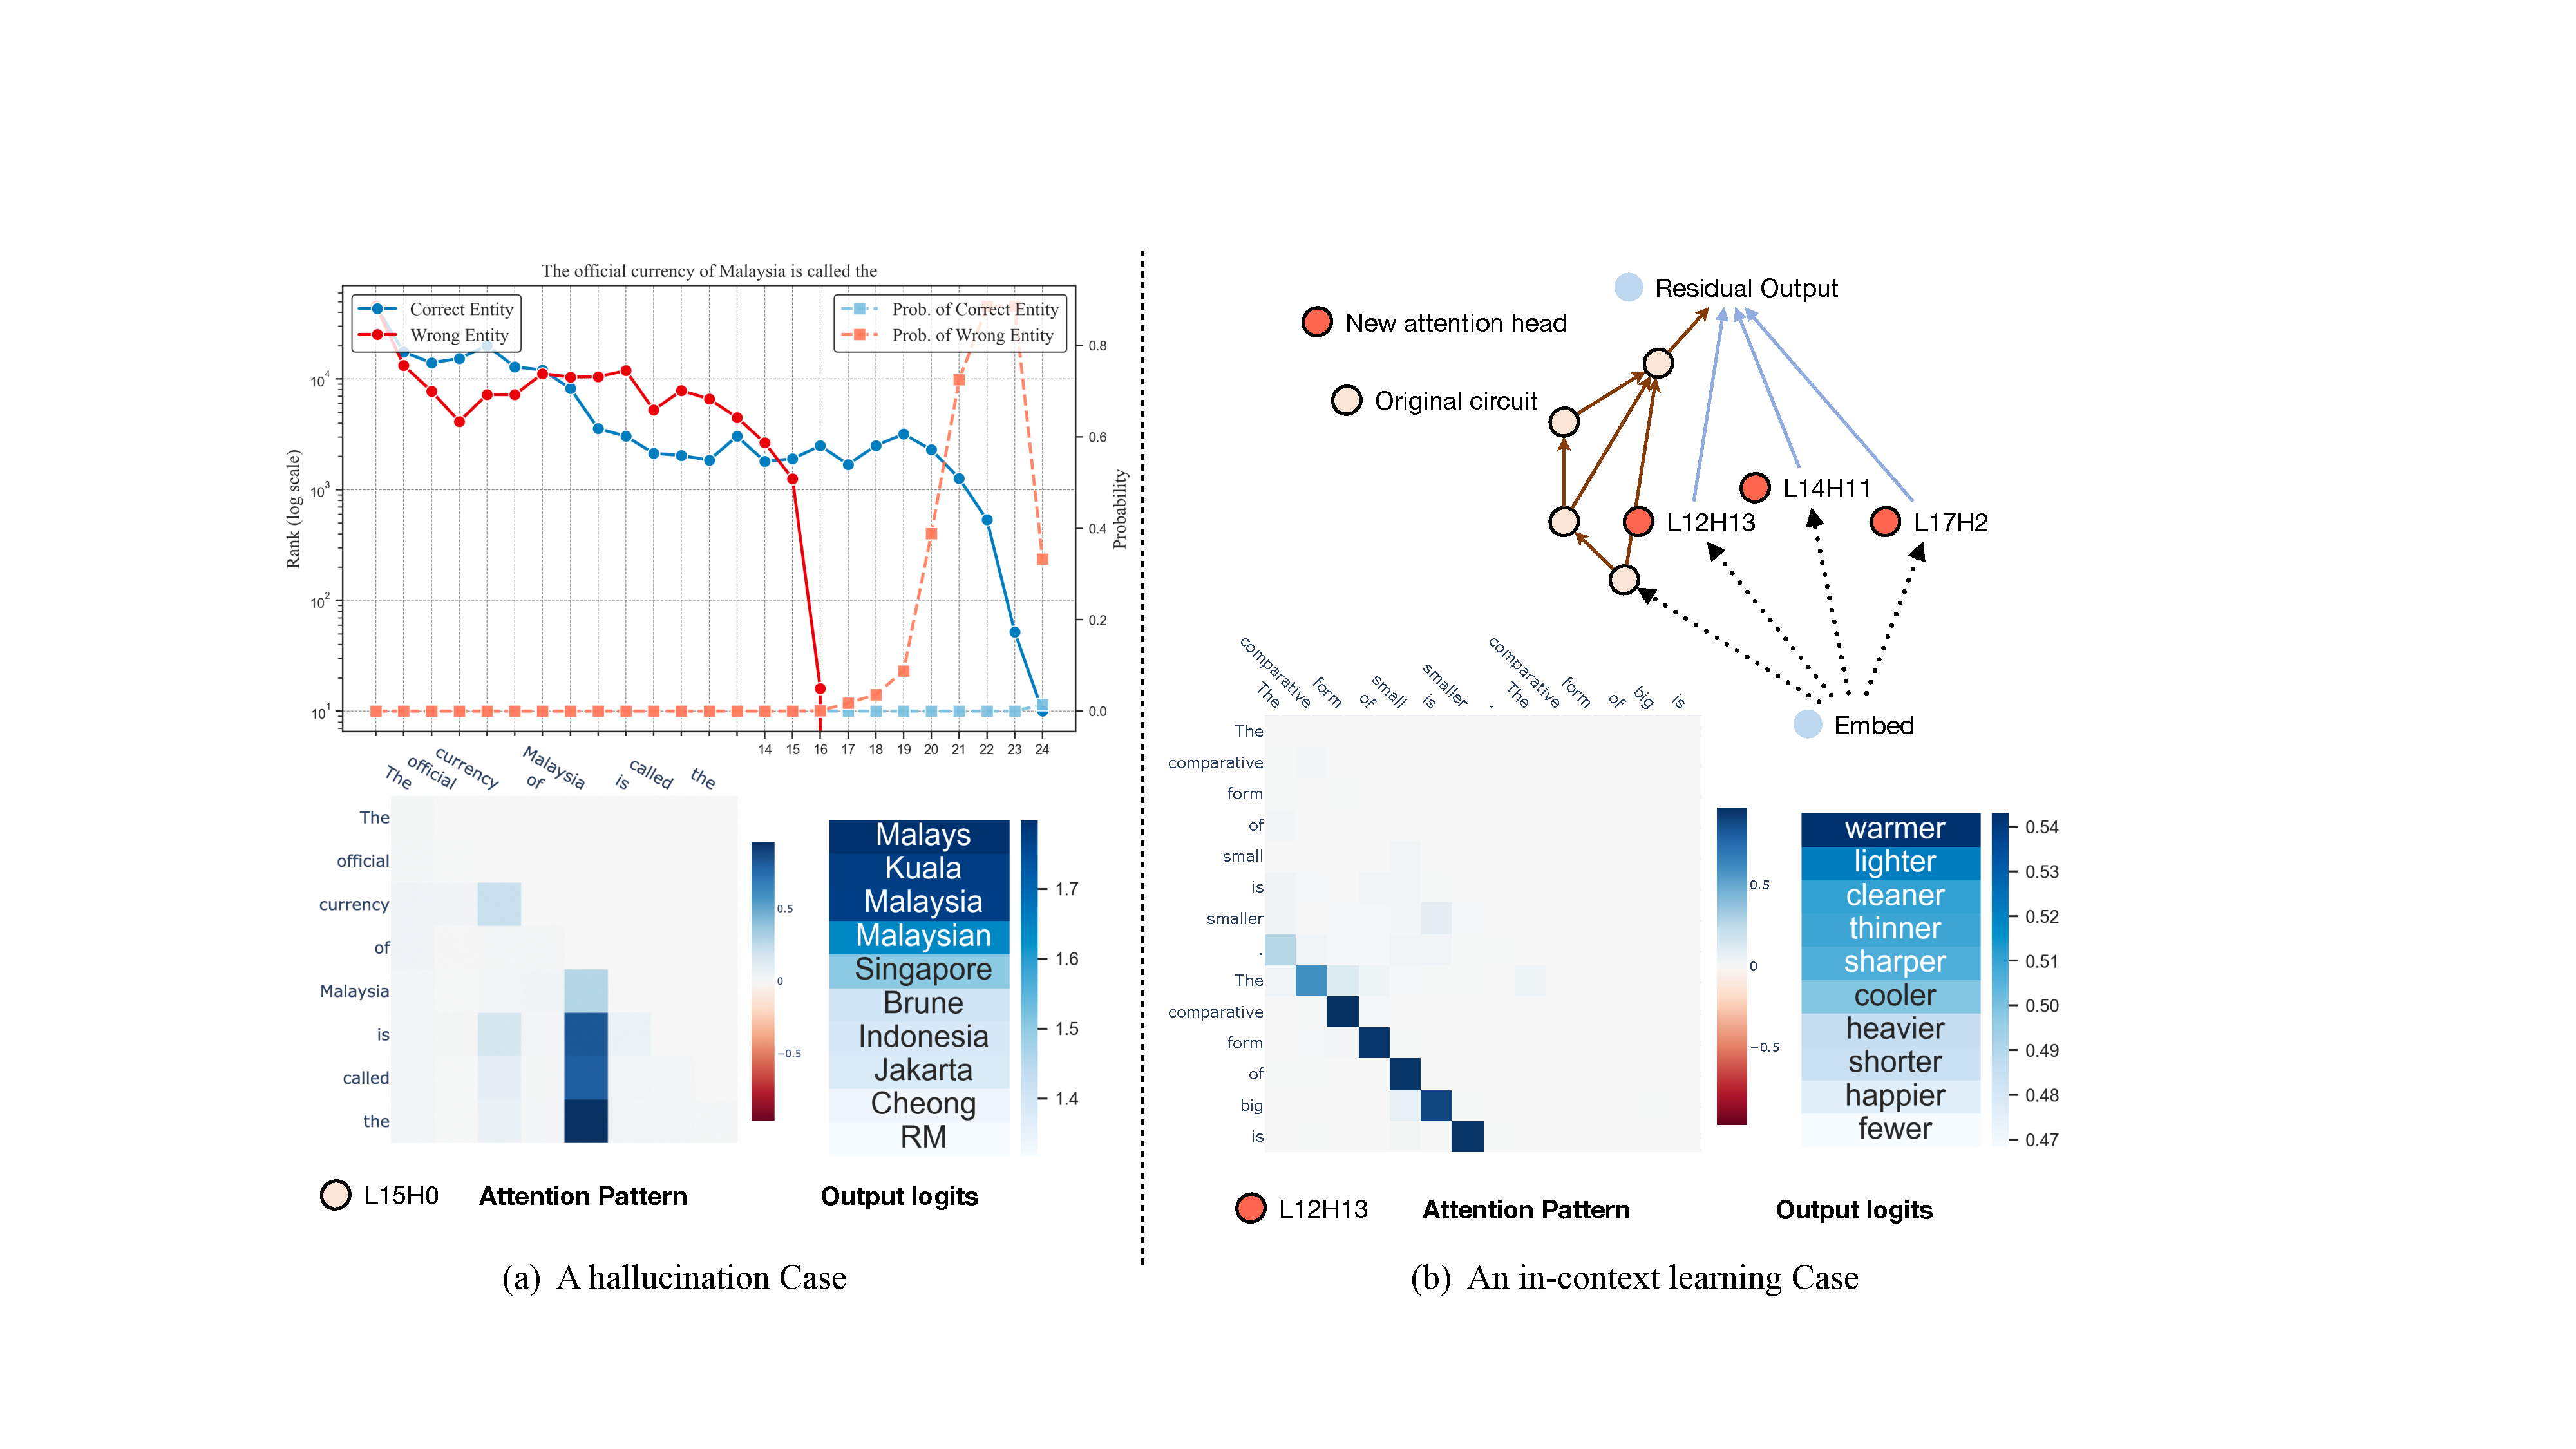
\includegraphics[width=0.99\linewidth]{Figure/hallucination.pdf}
    \caption{Left: fact hallucination case \nl{The official currency of Malaysia is called}, 
    we observe that, \textbf{at layer 15, the Mover Head selects incorrect information}.
    Right: In-context learning case, we notice that \textbf{some new heads focusing on the demonstration appear in the knowledge circuit}.
    %These heads would generate things that related to the format of the output.
    }
    \label{fig:hallucination}
\end{figure}

\section{Knowledge Circuits Facilitate Interpreting Language Model Behaviors}
% Locating shared circuits is a relatively new research topic, and only a few studies have investigated it.
In this Section, our aim is to validate whether the identified knowledge circuits are actually utilized by the model when it employs knowledge.
To address this, as shown in Figure \ref{fig:hallucination}, we investigate three phenomena: hallucination, in-context learning, and reverse relations (Details in Appendix~\ref{app:reverse_relation}).
\paragraph{Factual Hallucination.}
If the knowledge is stored and expressed by the circuit we discovered, we aim to discover what happened when the model gave us the incorrect answer.
We focus on factual hallucinations, which occur when the model provides an incorrect target entity for a given subject \(s\) and relation  \(r\).
In our experiments (Figure~\ref{fig:hallucination} and Appendix~\ref{app:sec_hallucination}), we observe that the model fails to move the correct knowledge to the final token in the earlier layers.
This failure is evident as the circuit lacks an effective mover head or the mover head selects incorrect information. 
For instance, in the prompt \nl{The official currency of Malaysia is called}, both the correct answer \nl{Ringgit} and the incorrect one \nl{Malaysian} are accumulated before layer 15. 
However, at layer 16, the mover head L15H10 extracts the erroneous information. 
Despite a rank drop of the true one in layers 20–22, this is insufficient to correct the previous mistake.
% Here, we compute two circuits: the circuit of the model that provides the incorrect answer and the circuit for the correct answer to see the difference between them.
\paragraph{In-Context Learning.}
Despite storing a vast amount of knowledge, a language model may still provide incorrect answers. 
However, with demonstrations or examples (based on RAG \cite{DBLP:journals/corr/abs-2312-10997}), it can quickly generate correct responses.
To this end, we focus on the scenario where the model initially provides an incorrect answer but can then produce the correct response upon receiving the appropriate demonstration. 
We consider the original knowledge circuit and introduce a new knowledge circuit based on the demonstration.
Our analysis reveals that, compared to the zero-shot knowledge circuit, several new attention heads appear in the computation graph when the demonstration is incorporated.
We show the behavior of these attention heads in Figure \ref{fig:hallucination}. 
We can see these heads mainly focus on the demonstration's context: \nl{The comparative form of small is smaller} and works as the Induction Head~\cite{olsson2022context} that look back over the sequence for previous instances of the current token and find the token that came after it last time.
To better view the function of these heads, we conduct experiments by ablating the newly appeared attention head in the ICL circuit in Table~\ref{tab:icl_ablate}. 
We find that compared to the randomly selected attention head by ablating this attention, the probability drops significantly in the prediction, demonstrating the importance of these identified attention heads.
These aligned with previous work where \citet{todd2024llms} have identified a concept known as the Function Vector, which represents the average of some key attention heads and provides the task learning ability.
% Please add the following required packages to your document preamble:
% \usepackage{multirow}
% \usepackage[table,xcdraw]{xcolor}
% Beamer presentation requires \usepackage{colortbl} instead of \usepackage[table,xcdraw]{xcolor}
% Please add the following required packages to your document preamble:
% \usepackage{multirow}
\begin{table}[ht]
\caption{Performance change via ablating the newly appeared attention heads in the ICL circuit and random heads.} 
\resizebox{\linewidth}{!}{
\begin{tabular}{llccc}
\toprule
   & \textbf{Knowledge} & \textbf{Origin Model} & \textbf{Ablating extra head} & \textbf{Ablating random head} \\ \midrule
Linguistic                   & adj\_comparative                       & 62.24                 & 32.55                   & 58.18                         \\  \midrule
\multirow{2}{*}{Commonsense} & word\_sentiment                        & 89.02                 & 55.50                        & 88.61                         \\
 & substance\_phase                       & 78.74                 & 52.85                        & 71.24                         \\ \midrule
Bias                         & occupation\_gender                     & 86.97                 & 59.54                        & 86.54                         \\ \midrule
Factual                      & person\_occupation                     & 35.17                 & 23.27                        & 31.60                         \\ \bottomrule
\end{tabular}
}
 \label{tab:icl_ablate}
\end{table}
% In our experiments, we found that these attention heads primarily focus on the demonstration, indicating their role in leveraging the demonstration to reactivate and correct the model's response.


% In addition to the function heads that we observe within the graph, we also notice that the output logits of the mover heads are significantly enhanced and we discuss this phenomenon in the Appendix~\ref{app:sec_few_shot}.
